% Tabela: Resultados do Experimento Delta
\begin{figure*}[!ht]
	\centering
		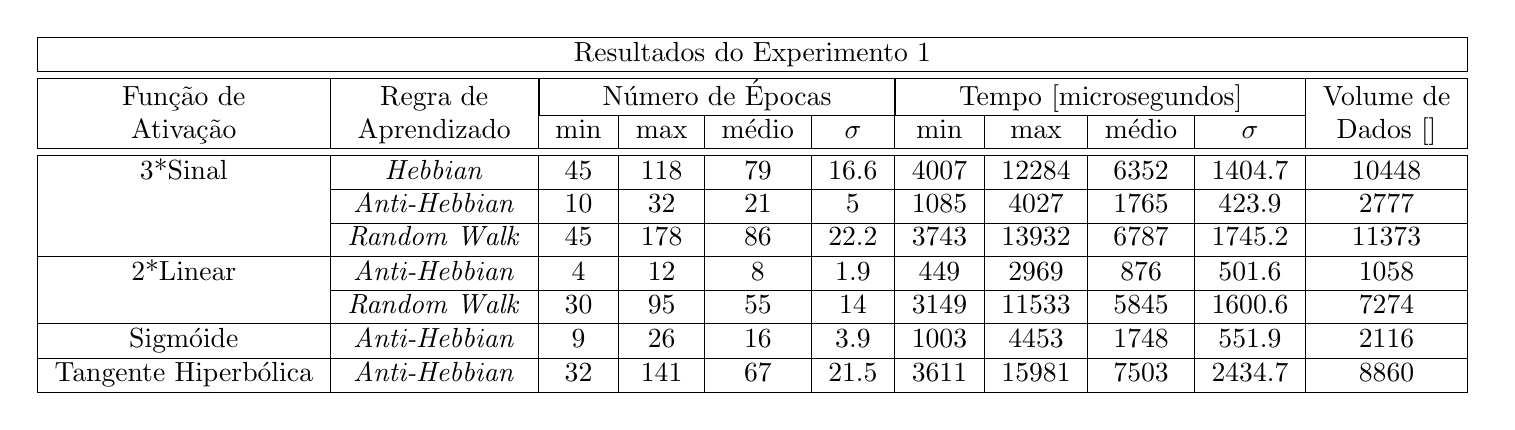
\begin{tikzpicture}
			
		\node[thick, align=center] (table) {
			\begin{tabular}{ |c|c|c|c|c|c|c|c|c|c|c| }
				\hline
				\multicolumn{11}{ |c| }{Resultados do Experimento 1} \\
				\hline \hline
				Função de &
				Regra de &
				\multicolumn{4}{ |c| }{Número de Épocas} &
				\multicolumn{4}{ |c| }{Tempo [microsegundos]} &
				Volume de \\ \cline{3-10}

				Ativação & Aprendizado & min & max & médio & $\sigma$ & min & max & médio & $\sigma$ & Dados [\Bytes]\\
				\hline \hline
				
				% Signal
				\multirow{3}{*}{Sinal} & \textit{Hebbian} & 45 & 118 & 79 & 16.6 & 4007 & 12284 & 6352 & 1404.7 & 10448 \\ \cline{2-11}
				& \textit{Anti-Hebbian} & 10 & 32 & 21 & 5 & 1085 & 4027 & 1765 & 423.9 & 2777 \\ \cline{2-11}
				& \textit{Random Walk} & 45 & 178 & 86 & 22.2 & 3743 & 13932 & 6787 & 1745.2 & 11373 \\
				\hline

				% Linear
				\multirow{2}{*}{Linear} & \textit{Anti-Hebbian} & 4 & 12 & 8 & 1.9 & 449 & 2969 & 876 & 501.6 & 1058 \\ \cline{2-11}
				& \textit{Random Walk} & 30 & 95 & 55 & 14 & 3149 & 11533 & 5845 & 1600.6 & 7274 \\
				\hline

				% Sigmoid
				Sigmóide & \textit{Anti-Hebbian} & 9 & 26 & 16 & 3.9 & 1003 & 4453 & 1748 & 551.9 & 2116 \\
				\hline

				% Hyperbolic Tangent
				Tangente Hiperbólica & \textit{Anti-Hebbian} & 32 & 141 & 67 & 21.5 & 3611 & 15981 & 7503 & 2434.7 & 8860 \\
				\hline
			\end{tabular}
		};

		\end{tikzpicture}
	\caption{Tabela de resultados do Experimento 1.}
	\label{tab:resultsDelta}
\end{figure*}